\section*{Problema 10}
\textbf{Considera el siguiente grafo:}
\begin{figure}[H]
    \centering
    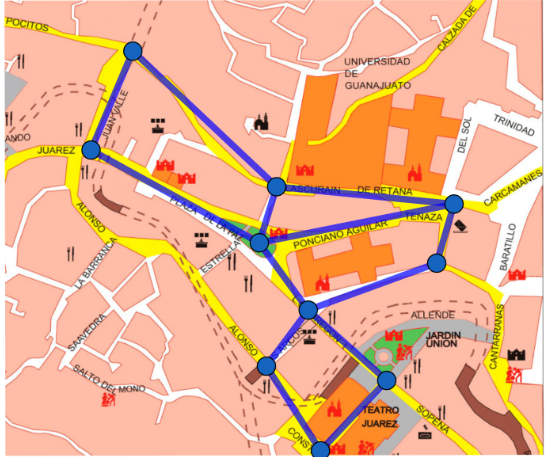
\includegraphics[width=8cm]{Graphics/problema_10.png}
\end{figure}
\textbf{Cada calle (arista) entre dos nodos esté bloqueda por una manifestación con probabilidad p. Supongamos que todos son eventos independientes.}
\subsection*{Problema 10a}
\textbf{Calcula la probalidad de poder caminar desde la puerta trasera del Teatro Juarez (nodo más abajo) al café conquistador (nodo más hacia arriba).}
\subsection*{Problema 10b}
\textbf{Decimos que un nodo del grafo está aislado si todas las aristas que llegan (o salen) están bloqueadas. Calcula el promedio del número de nodos aislados.}